%
% latex-sample.tex
%
% This LaTeX source file provides a template for a typical research paper.
%

%
% Use the standard article template.
%
\documentclass{article}

% The geometry package allows for easy page formatting.
\usepackage{geometry}
\geometry{letterpaper}

% Load up special logo commands.
\usepackage{doc}

% make a reference to Hypertext 
\usepackage{hyperref}

% Package for formatting URLs.
\usepackage{url}

% Packages and definitions for graphics files.
\usepackage{graphicx}
\usepackage{epstopdf}
\DeclareGraphicsRule{.tif}{png}{.png}{`convert #1 'dirname #1'/'basename #1 .tif'.png}

%
% Set the title, author, and date.
%
\title{\textbf{Descriptive and Predictive Analysis of Internet Rankings of Popular Music} 
\vspace{3mm}
\\ \small{DNSC 6211: Programming for Analytics}}
\author{
	Andrew Nichols \\
	Jessica Smith \\
	Yahui Zhou \\
}
\date{}

%
% The document proper.
%
\begin{document}

% Add the title section.
\maketitle

% Add an abstract.
\abstract{
\noindent
\normalsize
In the digital age it is easier than ever to discover new music. Users aren't limited to radio; they can share songs on Twitter and other internet platforms, subscribe to digital providers like Spotify, even identify any song they hear with the click of a button using the Shazam mobile app. Our group wanted to know whether these types of emerging data could be harnessed to answer questions of value to music industry executives, such as:

\begin{itemize}
\normalsize
\item Which ranking services are the most effective at tracking popular music trends?

\item Do tools to accurately forecast future hits currently exist?

\item What geographic areas tend to produce talented artists?
\end{itemize}

\vspace{1mm}
\noindent
\normalsize
To answer these questions we used web scraping to pull data from Billboard and Shazam's popular music ranking charts. In addition, we discovered an application programming interface (API) with information regarding artist's hometowns. We used our sources to produce data visualizations and an R Shiny application aimed at answering these questions. 

\vspace{1mm}
\noindent
\normalsize
We believe that our insights will be useful to music industry executives, and that the project could be expanded to provide even more value. This forecasting ability could provide significant value to individuals in the entertainment or marketing industry. \vspace{3mm}

\noindent
Our project is available on GitHub at \url{https://github.com/JASmith0820/Song_Rank_App}.\vspace{1mm}

\noindent
Our published R Shiny application appears at \url{https://jasmith0820.shinyapps.io/Song_Rank_App}.
}

% Add various lists on new pages.
\pagebreak
\tableofcontents


% Start the paper on a new page.
\pagebreak

%
% Body text.
%
\section{Introduction}
\label{introduction}

Our primary objective in completing this project was to become more proficient at using data science tools to access, process, and analyze data from the Internet, and to develop an online tool users could employ to assess the accuracy of popular music hit predictors.  Readers may be aware that several often-visited websites such as Billboard and Shazam provide real-time rankings of popular modern music, and sometimes try to predict which songs will be future hits.  We decided to pull data from several of these websites, and compare hit rankings, with the objective of developing a more effective and accurate way to predict hit songs.  Our data reflect some Twitter sentiment analysis through Twitter's influence on Billboard music rankings, and we present graphics that indicate where the most popular artists are from. This report outlines our decision-making process for the project, sources of data, methods of analysis, and success in creating some interactive online applications useful for comparing the rankings of hit songs.  Future work could exploit our lessons-learned, and create a song hit predictor that is better than any tool available today.

\section{Background}

\underline{Selection of the Data Set}:	Our team spent several hours evaluating the pros and cons of several online datasets like sports team records, stock and bond price data, movie hit rankings, Twitter feeds, and unemployment data.  We ruled out these data sets primarily because we thought it would not be possible to fulfill all of the requirements of the project using them. Music industry song rankings seemed both interesting and useful for making predictions, so we decided to exploit it.\vspace{2mm}

\noindent
\underline{Nature of the Data}:  The primary music industry data we used included the name of the most popular songs, the name of the artists who perform each one, and each song's rank according to the information provider.  The specific data sets we scraped to obtain data included:  the \href{http://www.billboard.com/charts/hot-100}{Billboard Hot 100}, \href{http://www.shazam.com/charts/top-100/united-statess}{Shazam Top 100}, \href{http://realtime.billboard.com/?chart=trending140}{Billboard Top Trending 140}, and \href{http://www.shazam.com/charts/future-hits/united-states}{Shazam Hit Predictor} (20 songs).  These sites calculate song rankings using unspecified formulas based on the frequency of radio airplay, music sales data, and streaming data from online music sources. \vspace{2mm}

\noindent
\underline{The Research Questions and How They Changed}:  Initially, we thought we could scrape music ranking websites and then mine Twitter data to see if Twitter's music-related chatter could help us develop a better predictor of hit songs.  As we pulled and saved the song data, however, we realized some of the titles were especially brief (examples like "Hello" by Adele), making it difficult to associate the songs with Twitter chatter about them.  As we encountered this complication, we began to focus more on what we could do with just the song ranking data already available from Billboard.  The most obvious thing to do was to plot the various rankings in two dimensions, as we ultimately did, to compare the sites' different methods for developing song lists.   



\section{Method}

The primary question driving our research was: what tools could a music executive (or other entertainment-industry stakeholder) use to understand and forecast trends in the music industry? For decades, Billboard has been recognized as the industry's primary source for popular music rankings, but are there new organizations that have better utilized emerging technologies to build better ranking mechanisms? For example, the popular mobile app Shazam allows users to determine the name of any song they hear by holding their phone up as a song plays. Shazam gathers an enormous amount of data, and claims to be able to predict future hits based on users' data. Therefore, a critical sub-question was whether or not Shazam's predicted hits did in fact go on to become hits at a later date. Twitter chatter can also serve as a bellwether for emerging trends. We wished to assess whether or not Twitter could be harnessed as a predictive tool for future hits. Initially, we planned to mine their data ourselves, but we quickly realized Billboard had already invested significant resources in similar data mining activities, so we choose to build upon their efforts rather than start from scratch. \vspace{2mm}

\noindent
A final question we wished to answer was whether or not a relationship exists between Billboard song popularity and album/MP3 sales. Unfortunately, we learned that sales data is rarely made public, probably because the corporations selling music have a business interest in keeping the data private. However, we learned that the Billboard rankings do include sales data collected by Nielson Music as part of their predictive algorithm, and so we were comfortable using their rankings even though we could not tie the rankings directly to sales data.



\section{Organization}

The three group members - Andrew Nichols, Jessica Smith, and Yahui Zhou - worked in a highly collaborative way, side-by-side, for virtually the whole project development process.  There was a project lead for each of the following areas, but we all worked together on each aspect of the project:


\begin{itemize}
\item Web Scraping - Jessica Smith

\item Code Integration and Testing - Jessica Smith

\item Graphics development - Yahui Zhou

\item API for Artist Data - Yahui Zhou

\item Plotting and ggplot2 - Andrew Nichols

\item Shiny Application Development - Andrew Nichols

\item Write-Up and Presentation - Andrew Nichols, Jessica Smith, and Yahui Zhou

\item GitHub - Jessica Smith
\end{itemize}


\subsection{Workflow}

\noindent
To recreate our project, you must run the files in the order specified in the workflow. The first step is to run the Python code, which contains many comments documenting the code. The first section scrapes the Billboard and Shazam websites, and stores the results in csv files with the name of the ranking service and the date. The code's second section takes historical files and loads them into a cumulative MySQL database. In the third section, the code performs several queries on the database, and stores the result in csv files. In the fourth and final section, the code uses an API service to determine the hometown of popular artists.\vspace{2mm} 

\noindent
In the second step, the csv files generated in step 1 are turned into plots using R. Running the R code (provided) will export the graphs to your working directory. The second step also takes the artist hometown data and plots it on a map of the world. \vspace{2mm} 


\noindent
Finally, in the third step, the plots created in the second step are showcased in an interactive Shiny application. You may use the “Run App” feature in R Studio to display the app as long as your working directory contains the ui.R and server.R files. You must also ensure that you have the Shiny and ggplot2 packages loaded on your machine for the Shiny app to function properly. 
\vspace{5mm}
\begin{figure}[hb]
  \centering
    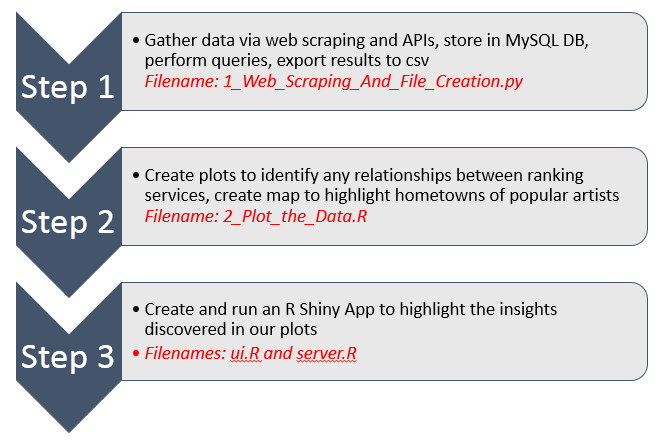
\includegraphics[scale=0.6]{Workflow}
  \caption{The project workflow}
\end{figure}

\subsection{Project structure}
Our sources included four music ranking websites and one artist information API. The ranking sources included the Billboard Hot 100, the Billboard Trending 140 in the Last 24 Hours, the Shazam Top 100, and the Shazam Hit Predictor. The Billboard Hot 100 draws from Billboard's experience and expertise, and ranks songs using a combination of radio airplay impressions and sales data from Nielson Music, as well as metrics derived from online streaming data. The Billboard Trending 140 provides real-time rankings of the most-shared songs on Twitter in the past 24 hours. The Shazam Top 100 shows the most popular songs among users of their mobile app. The Shazam Hit Predictor shows the 20 songs firm executives expect to be hits in the future based on data from their users. Shazam does not share the specifics of their algorithm. Note as well that these four sources primarily measure the popularity of music in the United States. The detailed analytics concept is in the diagram in the next page.\vspace{2mm}


\noindent
Comparing the Shazam Top 100 to the Billboard Hot 100 helped us understand whether or not the emerging Shazam technology reveals the same rankings as the industry standard (Billboard). In addition, by comparing the Shazam Hit Predictor and the Billboard Trending 140 to the Billboard Hot 100 one week later, we were able to evaluate the predictive powers of these two music ranking services. \vspace{2mm}


\noindent
Finally, the API providing artists' personal information allowed us to visualize the regions of the world from which the most popular artists are emerging. An industry executive could use this information to improve efforts to spot up-and-coming artists. See \url{https://github.com/echonest/pyechonest} for details about the API.

\vspace{25mm}
\begin{figure}[hp]
  \centering
    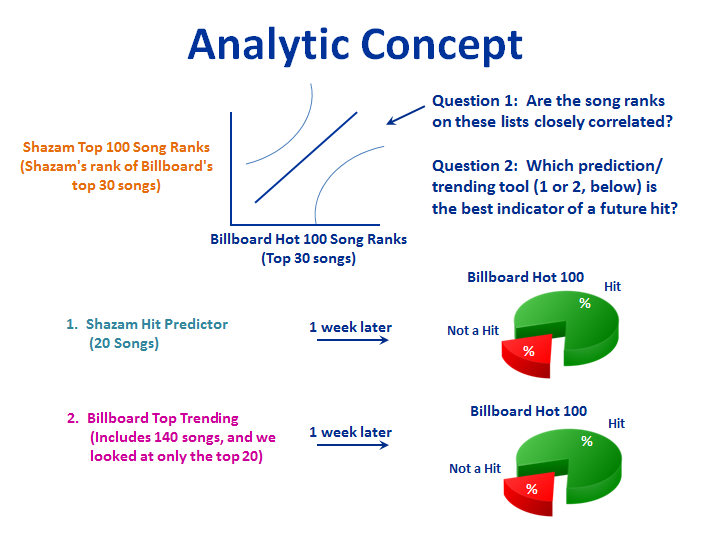
\includegraphics[scale=0.8]{Analytic_Concept}
\end{figure}

\subsection{Figures and Tables}

Figure 2 (below) compares Shazam Top 100 to Billboard Hot 100 rankings. Shazam rankings do not appear to correlate closely with the Billboard rankings. This is likely to be because Billboard incorporates a variety of factors into their rankings, including sales data and radio airplay impressions. Since Shazam's ranking process appears not to take such a multi-faceted approach, it is likely that they cannot gauge music popularity as accurately as Billboard can. Therefore, music popularity rankings on Shazam are not necessarily a good indicator of nation-wide popularity.\vspace{2mm}  

\noindent
In Figure 3, we have compared the 20 songs predicted by Shazam to be future hits against the Billboard Hot 100 from the following week. Only 30\% of the twenty songs made it onto the Billboard Hot 100, indicating that the Shazam hit predictor is not a particularly strong predictive tool, at least in the near term. In the future, it might be beneficial to perform an analysis similar to what we have done over a longer period of time to determine whether or not the songs become hits over a longer period of time.\vspace{2mm}

\noindent
In Figure 4, we are comparing 20 of the Billboard Trending 140 (the most-shared songs on Twitter) against the Billboard Hot 100 list from one week later. Many songs do appear on the Billboard Hot 100 (75\% of the top 20 Trending songs), indicating this list might be a useful tool for predicting upcoming hits. A song's position on the Trending 140 is not as important -- for example, Adele's "Hello" was number 15 in the top trending chart, but number 1 in the Billboard Hot 100. The Trending 140 is a real-time chart, and its hits often move slightly up or down in a matter of minutes. Therefore, a song's rank on the Trending 140 may not provide much information about where on the Hot 100 the song will appear, but simply appearing on the Trending 140 is an indicator that a song may be on the Hot 100 in the near future.\vspace{2mm}  

\noindent
In the last graph, we show the hometown locations of several of today's most popular artists. Many are from the northeastern United States and neighboring Canada, and they tend to come from the coastal regions rather than from the middle of each country. This could mean that these areas are hotbeds of musical talent, or that not enough venues exist in the other areas of each country to productively incubate top musical artists. A small number of artists popular in the North America come from Europe. Talent scouts can use these data to aid their searches for new talent. 

\begin{figure}[hp]
  \centering
    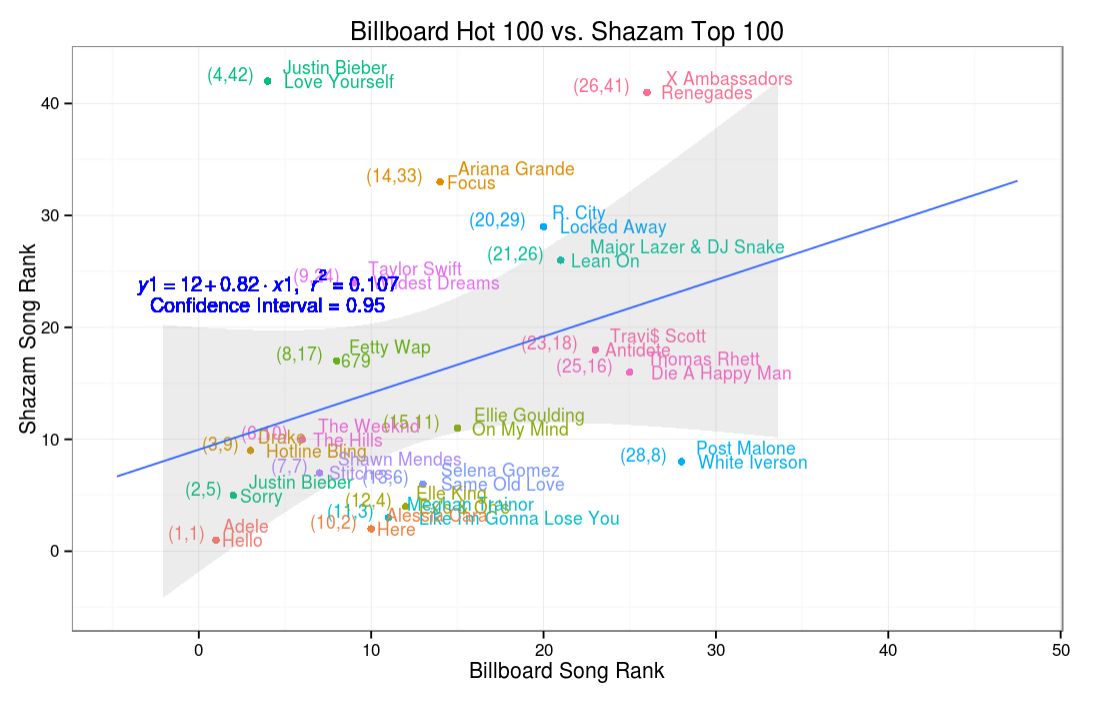
\includegraphics[scale=0.5]{2}
\end{figure}

\begin{figure}[hp]
  \centering
    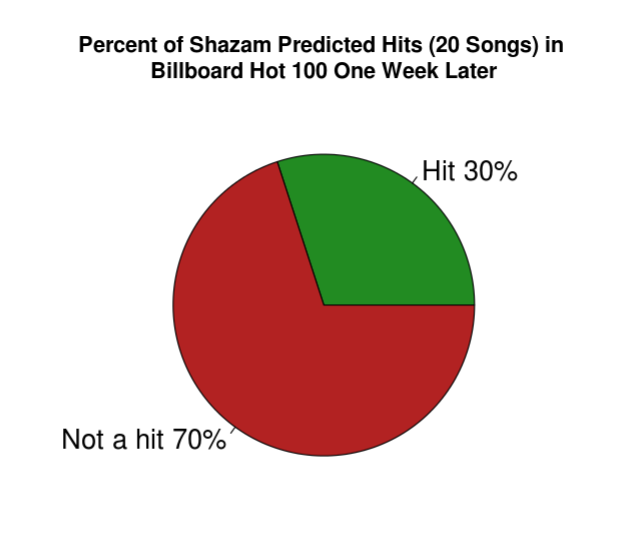
\includegraphics[scale=0.5]{3}
\end{figure}

\begin{figure}[hp]
  \centering
    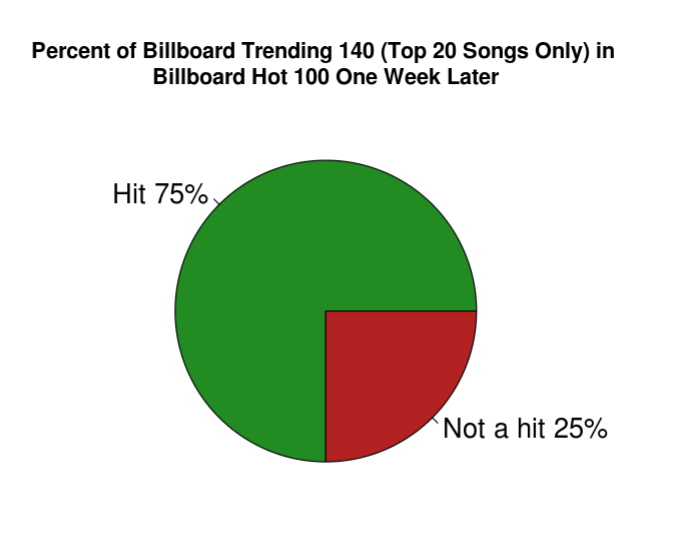
\includegraphics[scale=0.5]{4}
\end{figure}   
\begin{figure}[hp]
  \centering
    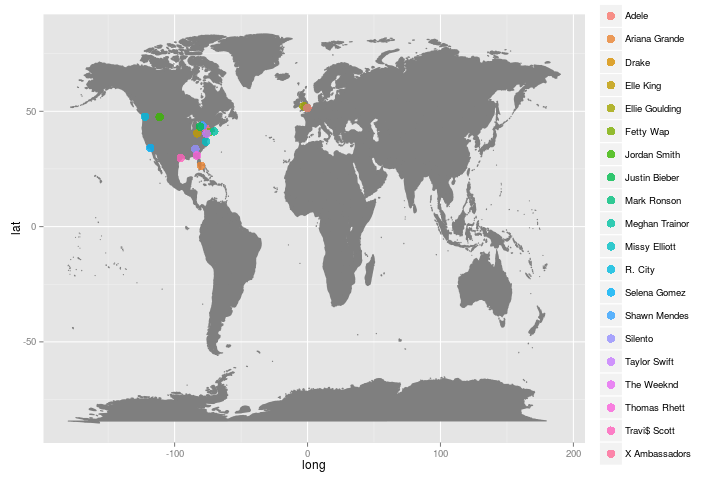
\includegraphics[scale=0.6]{ArtistMap}
\end{figure}


\section{Discussion}

Primary Selling Points:  The application we developed taught us two primary lessons about music rankings:  first, the Billboard hit predictor appears to be a much better predictor of future musical hits than the Shazam hit predictor.  Second, the top songs on the basic Billboard Hot 100 and the Shazam Top 100 lists are not as correlated as we expected them to be.  On the first point, in comparing the Shazam-predicted hits to those songs that actually made it onto the Billboard Hot 100, most of the Shazam predicted-hits never made it to the Billboard Hot 100 list (i.e., of 20 Shazam-predicted hits, only six made it to the Billboard list within one week's time).  By contrast, the Billboard Trending 140 list (which relies on Twitter data to identify popular songs), was a better predictor of Billboard's Hot 100 songs. \vspace{2mm} 

\noindent
An industry executive could use this information to keep track of emerging hits. Furthermore, this work could be expanded to cover a longer time frame, incorporate other lists (such as the Billboard Emerging Artist list or the Shazam Buzz list), and ultimately create a more robust hit predictor than the current industry offerings. 

\subsection{Lessons Learned}

Perhaps the most important lesson learned was the initial step of developing the project concept and thinking through the analytical or predictive value that might be obtained.  We believe we did a good job at this. We spent several hours evaluating different data sets we might use, and discussing what we could do with the data.  This enabled us to settle on one challenge (analyzing music industry data), and see the project through to completion relatively quickly.  We felt it was important to make our product interesting and useful to future users, and if possible, to create a better predictor of future hits. We have not yet developed a great song hit predictor ourselves, but we have developed several applications that users can employ to see and evaluate the performance of existing commercial predictors.  With time, we will likely discover indicators that will enable us to make more effective predictions ourselves.  Since we will all be taking follow-on courses together in data mining and forecasting, we discussed the possibility of continuing this project in the future as we learn more about predictive analytics.  \vspace{2mm} 

\noindent
This project allowed us to solidify our understanding of the technical skills we've covered in class, especially web scraping, storing and retrieving data from MySQL databases using Python, and creating visualizations in R. It was very gratifying to see something as "messy" as web data get cleaned up and converted into a clear and compelling data visualization.  


\subsection{Challenges}

The three main challenges for our project centered on the selection of the primary data set, the challenge of mining useful song-related information from Twitter, and the threat of being cut-off from API- or web-provided data for our project. As discussed above, we spent several hours working to identify a feasible and interesting data set. We ultimately settled on music industry information because it was readily available, it was amenable to data processing with the applications we were required to use, and we thought we could develop a better predictor of future hit songs. Other possible data sets (involving on financial data, sports, immigration, etc.) would have been interesting, but they are not always available and suitable for mapping and online interactive web applications. We initially planned to use Twitter data rather extensively, but it later became clear it would be hard to link Twitter chatter to sentiment regarding top songs because simple song titles like "Hello" and "Sorry" are very difficult to pick out in noisy Twitter data. In addition, much Twitter data about music involves people urging others to listen to their personal renditions of famous songs rather than on providing discernible sentiments about the famous songs themselves. The final challenge was that we were continually concerned that music websites might reorganize their interfaces (frustrating our scraping activities), or block us from an API we needed to determine where top artists were from.\vspace{2mm} 



\section{Conclusion}

In conclusion, this project afforded us an excellent opportunity to deepen our data gathering and visualization toolkit while producing a quality data science deliverable with inherent business value. We set out to scrape web sources for insights that would be useful to music industry executives, and we succeeded in drawing actionable conclusions from our sources. We determined that Billboard remains the music industry ranking standard for now, but that disruptive technologies like those employed by Shazam might dramatically change the competitive landscape. Fortunately for Billboard, the company seems to be ahead of its competitors in harnessing the power of resources like Twitter to identify emerging trends, as evidenced by the superior ability of the Billboard Trending 140 to predict hits over a 1-week time period as compared to the Shazam Hit Predictor. However, Shazam's data scientists might improve their predictive algorithm in the future, or other competitors might enter the market with even better algorithms. While our current project can provide useful insights to music executives, there remain many opportunities for continued developments along these lines. Now knowing the strength of the Billboard Trending 140, we could build a predictive model using this source, or we could continue to evaluate the strength of other available sources and ultimately develop an entirely new hit predictor ourselves.  The knowledge gained through this project has enabled us to understand and improve the predictive capabilities of a well-established and profitable international industry.


\end{document}

